\section{Anion Currents In The Human Atrium}

In a recent experimental study, Li et al.~\cite{Li2007} determined the existence
of a novel outwardly rectifying anion current in human atrial myocytes isolated
from right atrial appendages taken from patients undergoing coronary bypass
surgery.
A preliminary computational study has been conducted~\cite{Li2007}\ to
investigate the effects of the anion sensitive current, \ii{ANION}, on atrial
action potentials.
However it is still unclear on how this novel current affects intercellular
excitation conduction and cellular restitution properties.

It was known from the Li et al. study that influence on the atrial AP was small.
This study extended that to restitution properties and intercellular excitation
conduction.
It was expected that a small current would have a small influence on such
properties.
This would then have a small influence on the behaviour of spiral waves in two
dimensions.

\subsection{Methods}

The Li et al.~\cite{Li2007}\ study determined the current carried by this novel
ion channel, \ii{ANION}, could be modelled by
\begin{equation}
\label{eqn:anion:ianion}
I_{ANION} = g_{ANION} \frac{V-E_{ANION}}{1-\left(c\times e^{d\times\left(V-E_{ANION}\right)}\right)}
\end{equation}
where $g_{ANION}$ is the conductivity of the anion channel, $E_{ANION}$ is
the reversal potential of the channel and $c$ and $d$ are constants to
describe the behaviour.
All other symbols have their usual meanings.
They presented two sets of parameters for (\ref{eqn:anion:ianion}) given in
table~\ref{tbl:anion:params}, which described the current through the channel
when carrying a majority of \nothree\ or $\text{Cl}^{\text{-}}$ ions.

\begin{table}
    \caption[Parameter sets for the anion carrying current]{
        Parameter sets for the anion sensitive current \ii{ANION}\ when carrying
        \nothree\ and $\text{Cl}^{\text{-}}$\ ions.
    }
    \begin{tabular}{ l  c c}
    \toprule
    & \nothree & $\text{Cl}^{\text{-}}$ \\
    \midrule
    $g_{ANION}$ & 0.37   & 0.19 \\
    $E_{ANION}$ & -45.64 & -45.64 \\
    $c$         & 0.87   & 0.94 \\
    $d$         & $8.4\,\text{x}\,10^{\text{-4}}$ & $2.5\,\text{x}\,10^{\text{-4}}$\\
    \bottomrule
    \label{tbl:anion:params}
    \end{tabular}
\end{table}

This simulation study used the parameter set for the anion current carrying
$\text{Cl}^{\text{-}}$ ions.
The effects of the addition of this current to atrial myocyte cells was
quantified.
In the following paragraphs, `control' is used to denote the original
Courtemanche~et~al.~\cite{CRN98}\ atrial myocyte model and `anion' to denote the
Courtemanche~et~al. model with the addition current described by
(\ref{eqn:anion:ianion}) and using the $\text{Cl}^{\text{-}}$ parameter set from
table~\ref{tbl:anion:params}.

The effect on the behaviour of the cells caused by the anion current was
quantified using the simulation library described in
chapter~\ref{chapter:toolkit}\ for
control and anion cases.
As this simulation study was based on the CRN cell, the standard stimulus was
\ms{2} in duration and \unit{2}{nS} in magnitude.
Unless an alternative protocol is mentioned, all simulations directly followed
those described in Section~\ref{sec:toolkit:protocols}.

Simulating a single cell, the following measures were quantified: the AP
profile, the restitution of APD at 50\% repolarization, \apdr[50], the
restitution of APD at 90\% of repolarization, \apdr\ and the Effective
Refractory Period restitution, ERP\emph{r}.  The maximal fast sodium activation
was quantified at the same time as the \apdr\ was computed and is the product of
the three gates in \ii{Na}, as $m^{3}hj$. In all the single cell cases, the
cell was paced 10 times before the measurement was taken, to allow simulation
parameters to settle and to adapt to any changes in pacing rate.  Storage of the
cellular state was used in all appropriate points in the simulation, to minimise
computational time.

Using a 1D strand model the temporal Vulnerability Window to unidirectional
conduction block, VW, the Conduction Velocity restitution, CV\emph{r}\ and the
threshold of excitation were computed.  The strand model used was 300 nodes long
and had a space step of \mm{0.1}.  The diffusion coefficient, $D$, was set to
$0.03125\,\text{mm}^{\text{2}}\,\text{ms}^{\text{-1}}$~\cite{Biktasheva2005}.
In all 1D simulations the strand was paced 10 times before measurement was
taken.  In all simulations this state was then cached and restored as
appropriate, as described in the algorithms section of this chapter.

Using a 2D tissue model the lifetime of re-entrant spiral waves was estimated,
following the wave-break protocol outlined earlier.  The sheet had dimensions of
$375\times375$ nodes and a space step of \mm{0.1}.  The clamp potential used
to break the wave was \mv{0} and it was applied for \ms{1}.

\subsection{Results}


\begin{figure}
\begin{center}
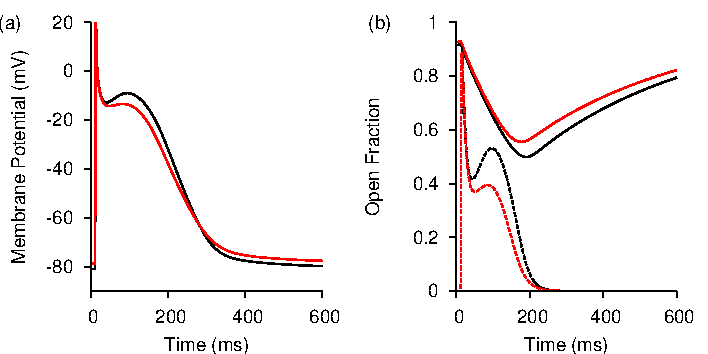
\includegraphics{figures/toolkit/anion/figures/01_AP}
\end{center}
\caption[Anion Current AP Profiles and \ii{Ca,L}\ gating parameters]{
\label{fig:tookit:anion:ap}
(a) AP profile for the CRN model in control (black) and anion (red) cases.
The inclusion of the $\text{Cl}^{\text{-}}$ carrying current results in a small
change of AP morphology, with a depressed plateau potential and an elevated
resting potential.
(b) Fractional opening of the gates of \ii{Ca,L}.
The $d$ (activation) gate is shown dashed, the $f$ (inactivation) gate solid.
Colours as in panel (a).
The $f$ gate takes longer to inactivate, whilst the $d$ gate does not activate
as much.
}
\end{figure}

The AP generated by the control and anion simulations are shown in
figure~\ref{fig:tookit:anion:ap}(a).
The \apd\ is slightly reduced from \ms{299.6} to \ms{297.3}, whereas the
\apd[50]\ is more significantly reduced, from \ms{180.1} to \ms{158.1}.
The AP profile shows a depressed plateau region (phase 2), reduced from
\mv{-9.56}\ to \mv{-14.1}\ and a slightly elevated resting potential,
\mv{-79.0}\ in the anion case cf. \mv{-80.9}\ in control.
This is consistent with the Li~et~al.~\cite{Li2007} study, and is included here
only for completeness.

Transients of the $d$ and $f$ gate of the \ii{Ca,L}\ open fractions are shown in
figure~\ref{fig:tookit:anion:ap}(b).
The $f$ gate in the \ii{ANION}\ case has a higher fraction of open channels for
longer than the control case.
The $d$ gate does not activate as much in the plateau region, contributing to
the shorter plateau.


\begin{table}
\caption[Calculated parameters for anion and control cells]{
\label{tbl:toolkit:anion_params}
Various calculated parameters for control (original CRN cell) and anion (CRN
cell modified to include $\text{Cl}^{\text{-}}$-carrying current).
The duration of the action potential at 50\% and 90\%
repolarization, \apd[50]\ and \apd\ respectively.
The maximum observed upstroke velocity of the action potential,
$\frac{dV}{dt}_{max}$.
The temporal vulnerability window to unidirectional conduction block, VW.
}
\begin{center}
\begin{tabular}{r l l l l}
\toprule
Case & \apd\ (ms) & \apd[50]\ (ms) & $\frac{dV}{dt}_{max}$ ($\text{mV}\,\text{ms}^{\text{-1}}$) & VW (ms)  \\
\midrule
Control & 299.6 & 180.1 & 217.1 & 3.22 \\
Anion & 297.3 & 158.1 & 210.6 & 3.94 \\
\bottomrule
\end{tabular}
\end{center}
\end{table}

The computed APD\emph{r}\ curves under the control and anion conditions are shown
in figure~\ref{fig:tookit:anion:apdr}(a) and \ref{fig:tookit:anion:apdr}(b), for the
restitution curves of APD at 50\% (\apdr[50]) and 90\% (\apdr) of repolarization,
respectively.
The
\apdr[50]\ shows the most significant differences, with the anion
curve depressed by \ms{20} even at the largest DI, increasing to a maximum
difference of over \ms{40} at at DI of \ms{380}.
The two curves then cross over at a DI of \ms{200}.
The \apdr\ curves, by contrast, are very similar for control and anion cases at
large (over \ms{600}) DI.
Between \msrange{100}{400}\ DI, the anion case is depressed compared to the control
case, with a difference of up to \ms{25}\ observed in the measured APDs.  At
\ms{100}, the curves rejoin one another and show a rapidly increasing slope as the
DI approaches \ms{0}.

\begin{figure}
\begin{center}
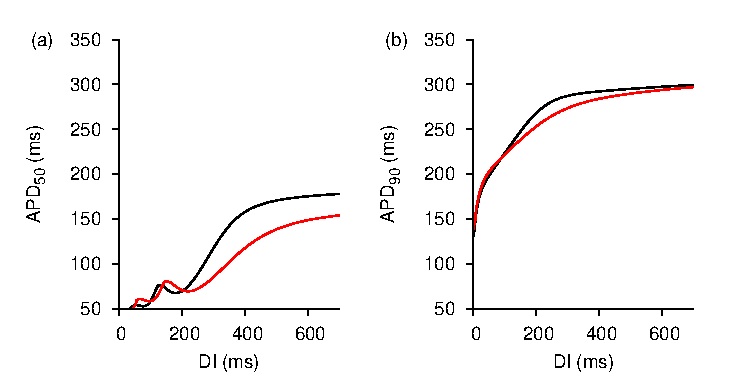
\includegraphics{figures/toolkit/anion/figures/02_APDR}
\end{center}
\caption[Anion Current APD Restitution]{
\label{fig:tookit:anion:apdr}
(a)
\apdr[50] curves for the CRN model in control (black) and anion (red) cases.
The two variants are different for all the DI in the simulation,
with the anion case below the control case for much of the DIs.
The slope is reduced by \ii{ANION}, compared to
the control case.  The curves cross at DI \ms{200}.
(b)
\apdr curves for the CRN model in control and anion cases.
The two variants behave the same at large DIs, but at decreasing DI the
anion case shows a greater reduction in the \apd.
At short DI (below \ms{100}) the two curves rejoin each other.
}
\end{figure}
\begin{figure}
\begin{center}
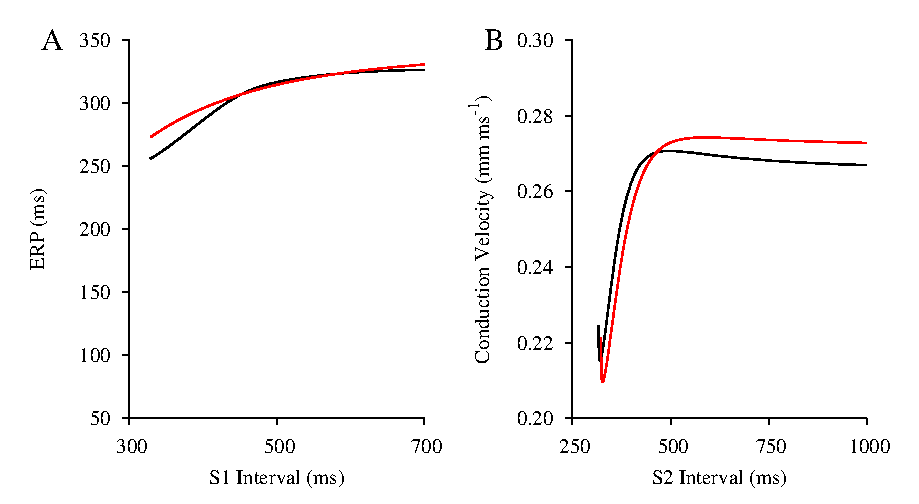
\includegraphics{figures/toolkit/anion/figures/03_ERPR}
\end{center}
\caption[Anion Current ERPr and CVr] {
\label{fig:toolkit:anion:erpr}
(a)
ERP\emph{r} curves for the CRN model in control (black) and anion
(red) cases.
The addition of the \ii{ANION} current changes the behaviour of the cell from a long
and flat plateau region followed by a relatively sharp decrease into a more
constant decline.
(b)
CV\emph{r}\ curves for the CRN model in control and anion cases.
 The CV\emph{r}\ curves are relatively flat for both cases over the range of
\msrange{500}{1000}, before they decrease rapidly in CV until the minimum
S2 interval is reached at approximately \ms{320}.
The CV is higher for the anion case at longer S2 intervals, before it
falls below control at an approximate S2 interval of \ms{460}.
}
\end{figure}

The ERP\emph{r} curves produced by the control and anion cases are shown in
figure~\ref{fig:toolkit:anion:erpr}(a).
In both cases the ERP\emph{r}\ curves are relatively
flat, decreasing by approximately \ms{60}\ over the \ms{700}\ range of S1
intervals considered.  The addition of the \ii{ANION}\ current changes the
behaviour of the ERP\emph{r} curve in a manner which is not simply a shift left
or right.  The control case shows a response which has a clear plateau region
which continues until an S1 interval of \ms{500}\ is reached and then a
relatively steeper decline until eliciting an AP of the appropriate magnitude
becomes impossible at an S1 interval of \ms{330}.  The anion case, by contrast,
shows a decreasing ERP over the whole range of S1 intervals considered although
it too shows its steepest slope just before eliciting a sufficiently large AP
becomes impossible, also at approximately \ms{330}.  At long S1 intervals (above
\ms{700}) the ERP\emph{r}\ is longer for the anion case before the curves cross
at \ms{600}\  and then again at \ms{450}\ with the ERP in anion at the point
where further stimulation becomes impossible almost \ms{20}\ higher than in the
control case.

The temporal VW increased with the addition of the anion current from \ms{3.22}
in control to \ms{3.94}\ in anion case, a 22\% increase in the size of the
region of unidirectional conduction block, shown in table~\ref{tbl:toolkit:anion_params}.
The CV\emph{r}\ curves, shown in
figure~\ref{fig:toolkit:anion:erpr}(b), suggest that tissue with the anion sensitive current
shows faster CV at normal physiological stimulus intervals (corresponding to
\msrange{500}{1000}).
The average conduction velocity with \ii{ANION}\ is
$0.274\,\text{mm}\,\text{ms}^{\text{-1}}$ in anion,
compared with $0.268\,\text{mm}\,\text{ms}^{\text{-1}}$ in control in this range
of S2 intervals.
As the conduction interval is reduced below \ms{500}, the conduction velocity
starts to decrease rapidly until conduction stops at \ms{323.4} for anion and
\ms{317.1} for control.
There is a brief recovery of conduction velocity visible in both cases, just
before conduction block.

\begin{figure}
\begin{center}
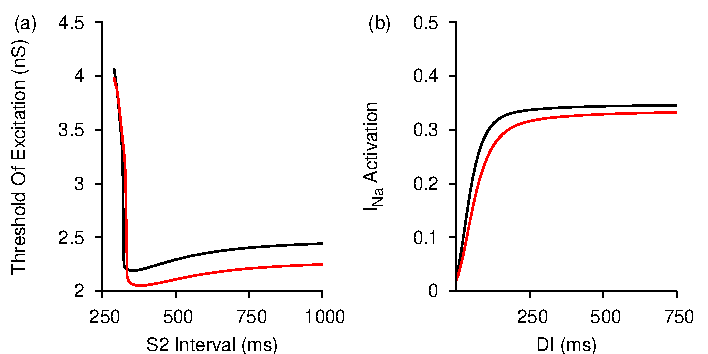
\includegraphics{figures/toolkit/anion/figures/04_ToE}
\end{center}
\caption[Anion Sensitive Threshold Of Excitation and \ii{Na} activation]{
\label{fig:toolkit:anion:toe}
(a)
Threshold of excitation curves in control (black) and
anion (red) cases.
As S2 decreases, so does the threshold of excitation until a critical point is
reached and the current which must be injected to reach the threshold almost
doubles.
In the control this comes at a $\Delta t$ of
\ms{321}\ and in anion at \ms{330}.
Until the critical point threshold of excitation is consistently lower for cells
with \ii{ANION}\ present.
(b)
Maximal activation of the fast sodium current, \ii{Na}, as DI is decreased.
The fast sodium current consistently activates to a greater degree in control
cases.
The effect is rate dependent with the greatest difference observed at DI \msrange{150}{200}.
}
\end{figure}

The threshold of excitation, shown in figure~\ref{fig:toolkit:anion:toe}(a), shows that
\ii{ANION} reduces the minimum stimulus current by approximately \unit{0.2}{nS},
a reduction of 10\%, at almost all $\Delta t$\ intervals.  It is also
interesting to note that both control and anion tissue types show `supra-normal'
excitability, with the minimum stimulus current decreasing as $\Delta t$\
decreases.  This occurs until a critical point is reached when the cell suddenly
becomes significantly harder to excite, with the minimum stimulus current
increasing almost 100\%.
This occurs \ms{9}\ later in control tissue at
\ms{321}\, compared with \ms{330}\ in control.

The maximal activation of the fast sodium current, \ii{Na}, is shown in
figure~\ref{fig:toolkit:anion:toe}(b).
The presence of \ii{ANION}\ consistently reduces the maximal activation of \ii{Na}.
At long DI, greater than \ms{400}, the reduction is 3\%, increasing to almost
twice that in the range of \msrange{150}{200}.
Both curves rapidly decrease to almost no \ii{Na}\ activation at an DI of
\ms{0}\ but the anion case starts this descent first.
\begin{figure}
\begin{center}
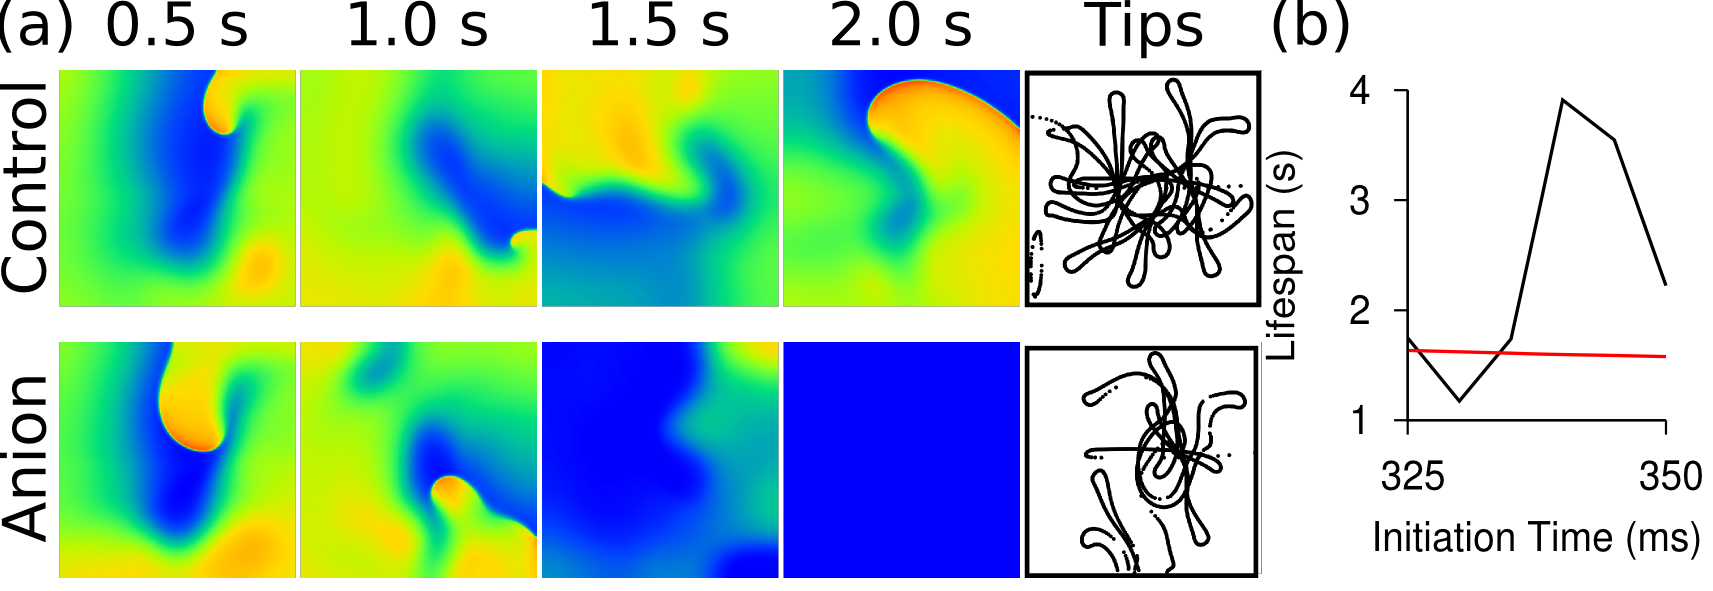
\includegraphics{figures/toolkit/anion/twod_traces}
\end{center}
\caption[Anion Sensitive Tissue Sheets and Spiral Lifespands]{
\label{fig:toolkit:anion:spiral}
(a)
Representative membrane potentials and tip trace for control (top row) and anion
sensitive cases (bottom row).
Times are from the initiation of spiral activity via cross--field protocol.
Cross--field stimulus was delivered at \ms{345}\ wall time.
Colour represents membrane potential and is coloured from blue (depolarised,
\mv{-80}) to orange (excited, $>\mv{0}$).
Both spiral waves are highly mobile, meandering over a very large area of
tissue.
(b)
Lifespan as related to time of initiation.
Lifespan in \ii{ANION}\ is relatively constant at around \ms{1600}\ whilst
control lifespan fluctuates considerably.
}
\end{figure}
Spiral waves were induced in a square sheet.
Representative plots of the
membrane potential over the whole sheet, produced as the simulation was ongoing,
are shown in figure~\ref{fig:toolkit:anion:spiral}(a).
The top row corresponds to control tissue, whilst the bottom row has an
\ii{ANION}\ sensitive current active.
Times of the membrane potential snapshots are relative to initiation of reentry at t = \ms{345}.
Tip traces are in the 5th column.
In both cases the spiral wave starts in the centre of the tissue and then follows a
looping track around the tissue before finally it exits the tissue when it
cannot turn fast enough around its own refractory tail.
Lifespans of reentry from differing initiation times are shown in
~\ref{fig:toolkit:anion:spiral}(b).
Lifespan in \ii{ANION}\ is relatively constant at around \ms{1600}\ whilst
control lifespan fluctuates considerably, from \ms{1175}\ to \ms{3910}.

\subsection{Discussions and Conclusions}

The effects of the inclusion of an anion sensitive current do not seem to be
that large, at least when considered on the single cell level.
However, despite the small influence of the current on the action potential duration,
it does have noticeable effects on the restitution properties of the cell and
on the behaviour of cells in a tissue.
The general behaviours of the Courtemanche cell have been discussed elsewhere,
for example in~\cite{CRN98,Cherry2008a}, I only discuss the differences the
\ii{ANION}\ current makes.

The most noticeable effect of the inclusion of \ii{ANION}\ in a cellular model
is the abbreviation of the \apd[50]\ and an accompanying reduction in the
plateau potential.  The abbreviation is due to \ii{ANION}\ acting as a
rectifying current when the membrane potential is above \mv{-45}.   Conversely,
at potentials below \mv{-45}\ \ii{ANION}\ acts to depolarize the cell, leading
to the slightly elevated resting membrane potential observed between action
potentials.  This difference in effect is what leads to the interesting
behaviours observed in cells with \ii{ANION}.

The \apdr[50]\ and \apdr\ curves show that \ii{ANION} has a rate dependent
effect.  Both curves are flattened in the cells which include \ii{ANION}\, but
this flattening is not uniform over the range of DIs considered.
\ii{ANION}\ has a simple exponential dependence on the membrane potential and no
time-dependent gating variables however, so it is not \ii{ANION}\ that causes
this rate dependence directly.
Instead, we must look to the currents active within the plateau region of the
action potential.
\ii{CaL}\ is the principle current responsible for the plateau region of the
action potential and unlike \ii{ANION} it has both time and voltage dependant
gating variables for activation, $d$, and inactivation, $f$.
The $d$\ gate is not as interesting as the $f$\ gate, as its time-course is not
affected by the presence of \ii{ANION}, although its activation during the
plateau region is reduced.
However, the $f$\ gate in \ii{ANION} cells never inactivates as completely as
it does in the control simulations which lack the current.

For the 1D strand results, both the CV\emph{r} and threshold of
excitation data also show rate dependent influence.
At a long stimulus interval, the increased excitability of the cell by the anion
current leads to a higher conduction velocity~\cite{Nygren2000}.
The increased excitability at long stimulus interval is due to the inward nature
of the anion current in the very first stages of the action potential.
This increased excitability allows atrial cells with \ii{ANION}\ to conduct the
excitation wave faster until, when the stimulus interval reaches a critical value of
\ms{500}, control cells start to conduct faster.
At this stimulus interval, the threshold of excitation is still lower for the
anion case, so another factor is responsible for the reduction in conduction
velocity.
The excitability of the cell is an important influence on the conduction
velocity, but it is not the only factor.
Another major factor is the upstroke velocity of the action potential which is principally
determined by the fast sodium current, \ii{Na}.
This is partially inactivated by the elevated resting potential in the anion
case, which also reduces the rate of recovery of the inactivation variables.
When the test stimulus is delivered after a reduced conduction interval in the
anion case \ii{Na}\ does not open as fully, slowing the upstroke and thus
leading to a reduced conduction velocity at short stimulus intervals, compared
with the control case.

The increase in the
vulnerability window appears to be quite significant, at over 20\% larger than
the vulnerability window in tissue without \ii{ANION}.
An increased vulnerability window has an obvious influence on the genesis of
re-entrant excitation---A larger vulnerability window increases the chance of a
premature excitation interrupting the normal function of the heart.
Though in both cases, the vulnerability window is relatively small.


Dynamic behaviours of the 2D spiral wave are interesting.
Both cells show a highly mobile spiral tip, due to their long \apd\ and ERP
relative to the size of the tissue.
However in the \ii{ANION}\ case, this does not translate into a widely varying
spiral lifespan, as might be expected from such mobility.
The restitution properties are generally slightly flattened by the inclusion of
\ii{ANION}, although perhaps importantly here, in the rapid pacing region, the
ERP is higher for \ii{ANION}\ bearing cells.
Further investigation, perhaps using the phase field
method~\cite{Biktashev1994}\ to start with a `stationary' spiral would be of use
to elucidate the effects.
